\PassOptionsToPackage{hyphens}{url}
\documentclass[compress,aspectratio=169]{beamer}

\usetheme{Reading}

\graphicspath{{../2019-06-isc/}{../2019-06-isc/fig/}{img/}{../logo/}}

\newcommand{\ok}[1]{{#1 (done)}}
\newcommand{\ongoing}[1]{{#1 (ongoing)}}
\newcommand{\started}[1]{{#1 (started)}}
\newcommand{\pending}[1]{{#1 (pending in plan)}}
\newcommand{\hrefb}[2]{\href{#1}{\textcolor{red}{#2}}}

\subtitle{}
\title{\Large  How to Contribute to the Certification Standard?}
\author{Julian Kunkel (+ HPC Certification Forum)}
\date{2020-05-20}
\authorURL{https://hpc-certification.org}
\authorFooter{Julian M. Kunkel et al.}
\venue{The HPC Certification Forum: YouTube Series}
\institute{Department of Computer Science}
\groupLogo{
\includegraphics[width=2.5cm]{hpccf-small}}
\titleLogo{ 
\includegraphics[height=2.5cm]{blur-book-stack-books-590493}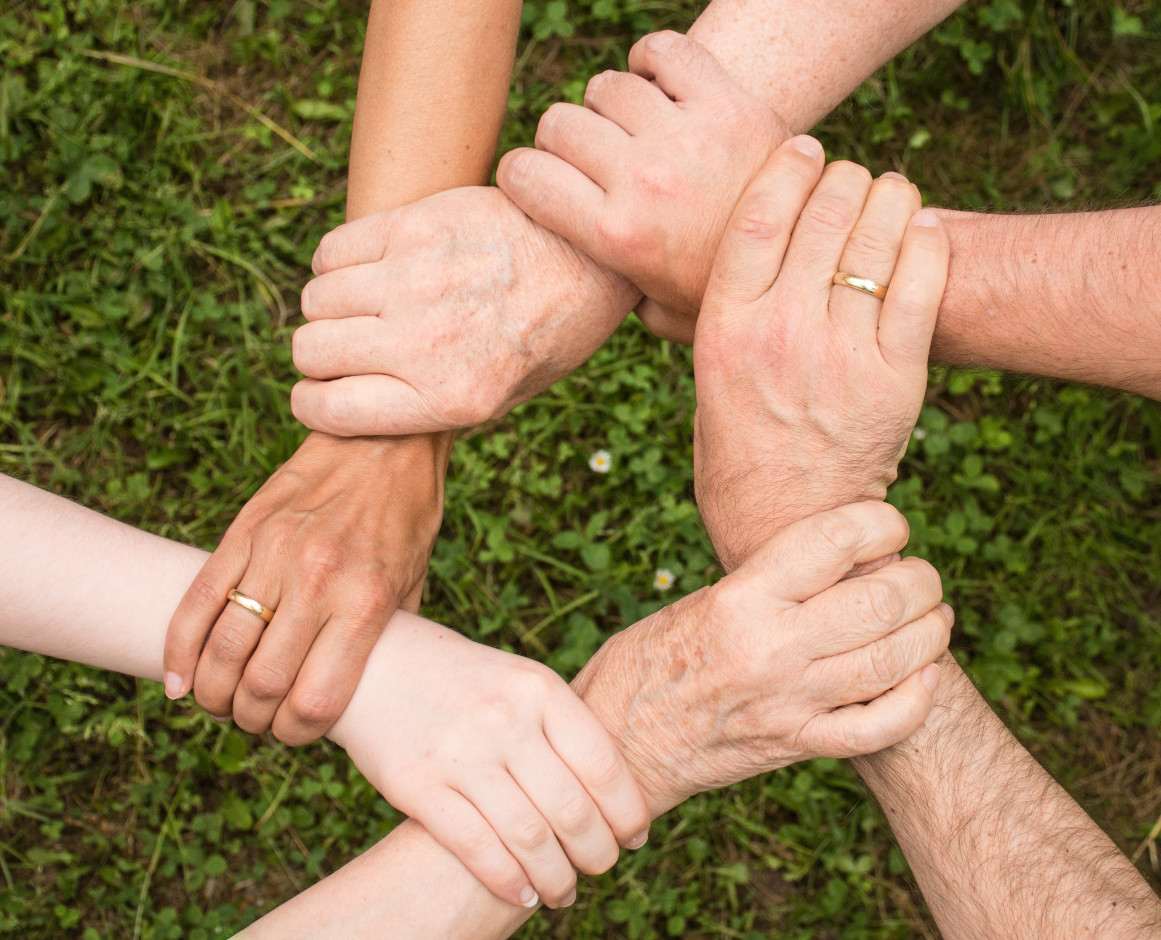
\includegraphics[height=2.5cm]{ground-group-growth-461049}
\includegraphics[height=2.5cm]{accomplishment-ceremony-college-267885}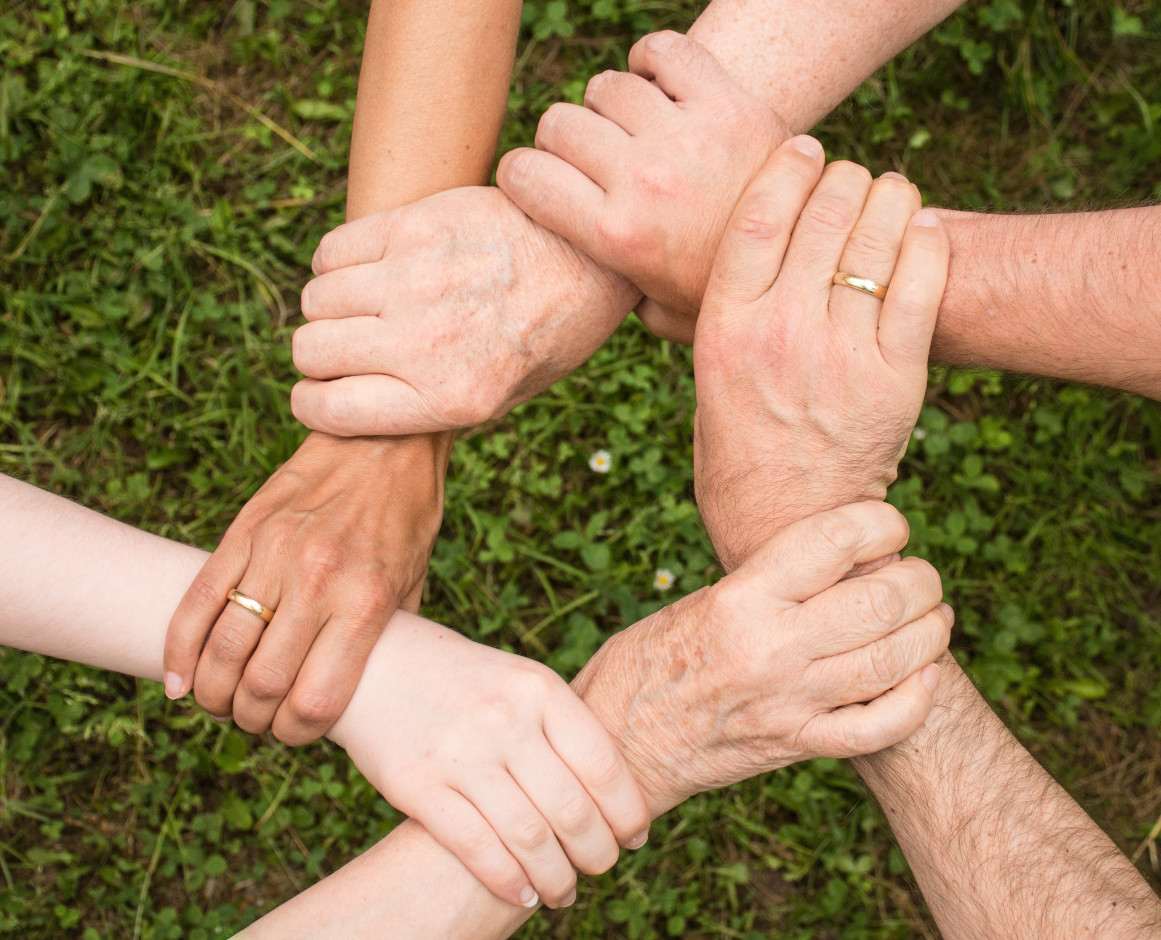
\includegraphics[height=2.5cm]{ground-group-growth-461049}
\includegraphics[height=2.5cm]{blur-book-stack-books-2}}


\begin{document}

\begin{frame}[plain]{}
	\maketitle
\end{frame}

\section{Learning Objectives}

\begin{frame}{Learning Objectives}
\begin{itemize}
  \item Describe the role of the HPC Certification Program
  \item Organize competences using a MindMapping tool
  \item Defining a skill using Markdown on GitHub
  \item Defining a skill using the Wiki
\end{itemize}
\end{frame}


\section{The Forum}
\subsection{}



\begin{frame}{The 
\includegraphics[width=0.45\textwidth]{hpccf-full}}
		\begin{block}{Goals}
			\begin{itemize}
				\item Standardizing the HPC knowledge representation into fine-grained competences
          \begin{itemize}
            \item What competences exist, how are they defined?
            \item Puzzle of competences for everyone (practitioners, students, admins)
            \item Supporting navigation and role-specific knowledge maps
          \end{itemize}
				\item Establishing international recognized certificates attesting knowledge
        \item Supporting an ecosystem around the HPC competences
			\end{itemize}
		\end{block}
\end{frame}


\section{Competence Standard}

\begin{frame}{The Competences Standard (CS) == Skills + Tree}
	\begin{itemize}
    \item The Competence Standard follows processes to evolve
		\item A \textbf{skill} defines background, objectives, learning outcomes
		\item The \textbf{skill tree} organizes the competences as hierarchical skills
	\end{itemize}

	\begin{figure}
		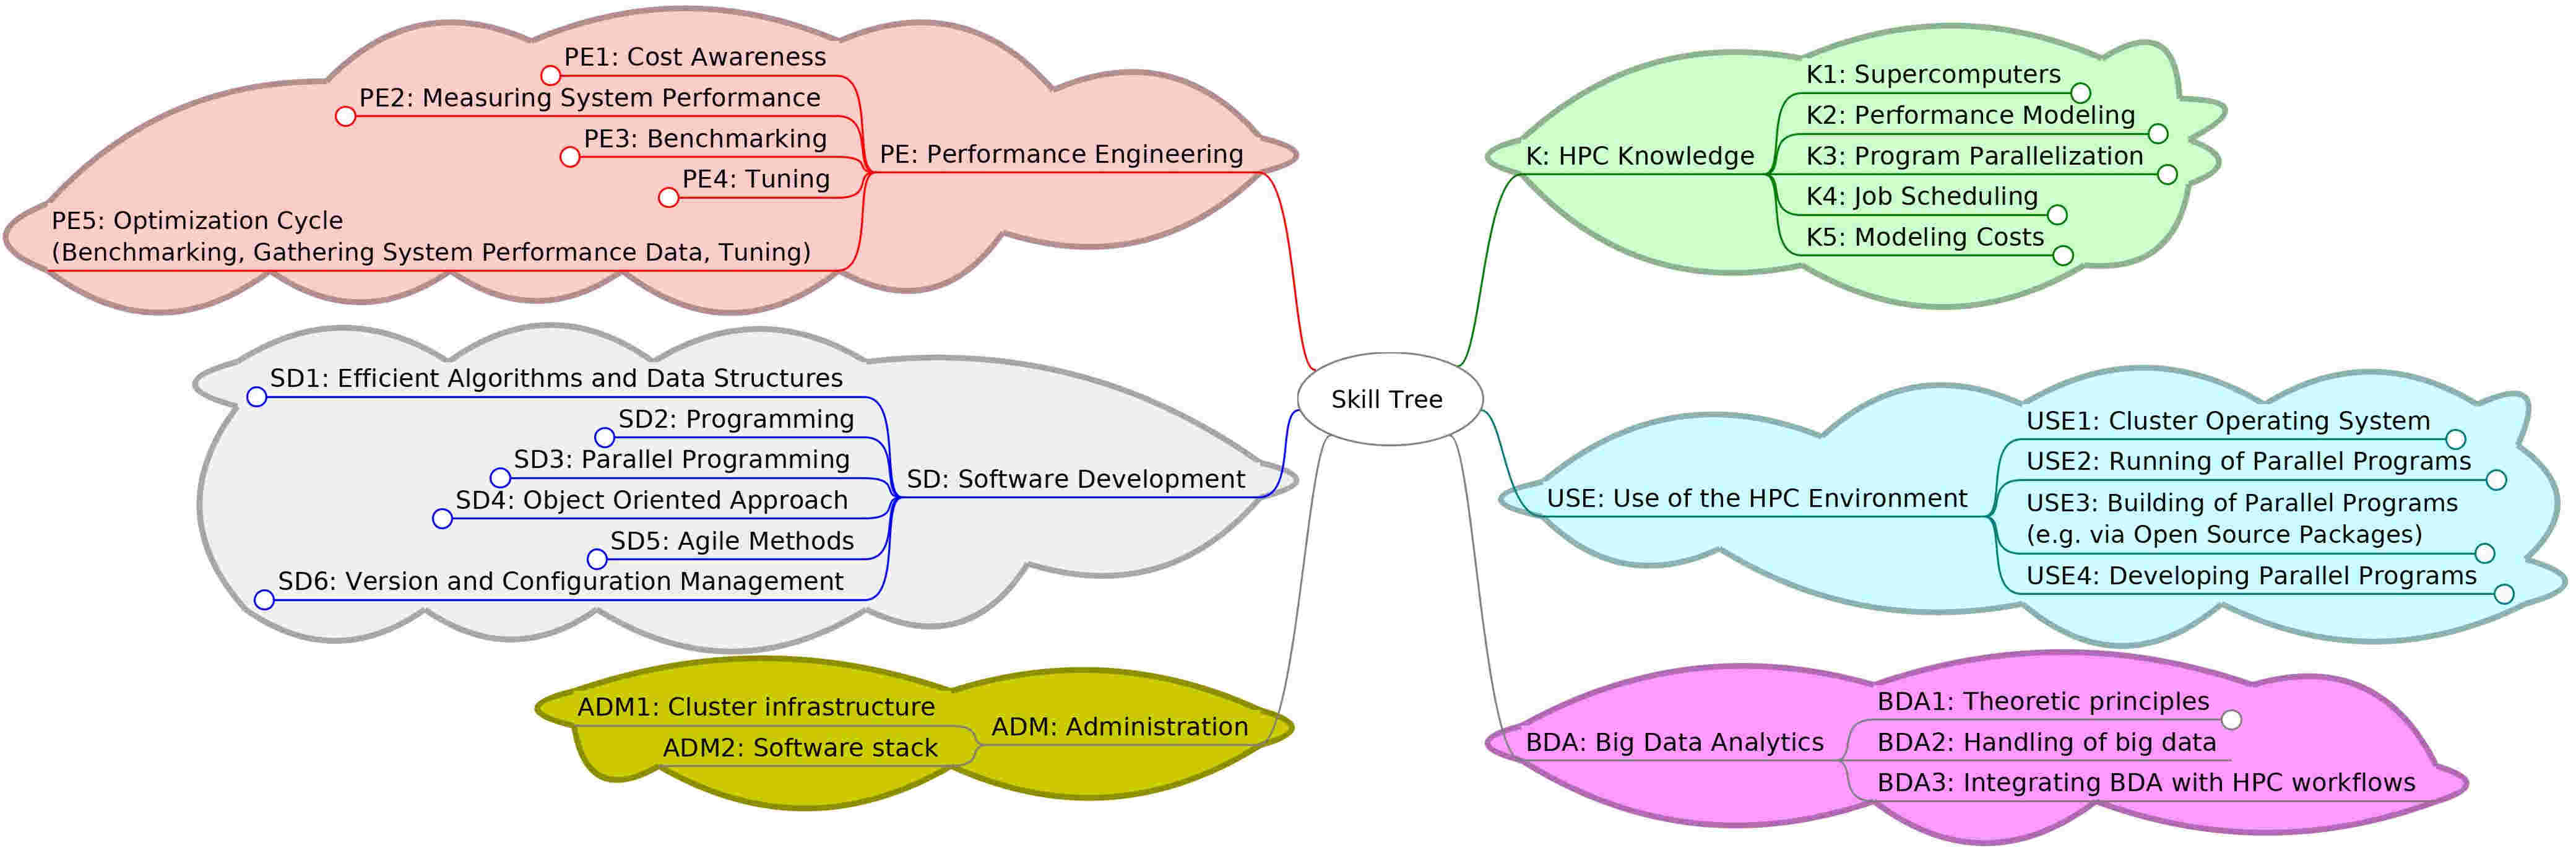
\includegraphics[width=\textwidth]{skill-tree}
		\vspace*{-2em}
		\caption{Top-levels of the skill tree (Initial ADM and BDA branches)}
	\end{figure}
\end{frame}


\begin{frame}{Example High-Level Skill (Excerpt)}
\begin{itemize}
\item Name: SLURM Workload manager
\item Id: USE4.2.2-B
\item Background: {\small SLURM is a widely used open-source workload
manager providing various advanced features.}
\item Aim:
\begin{itemize}
\item comprehend and describe the basic architecture of SLURM and its tools
\item use relevant tools to run and monitor (parallel) applications
\end{itemize}
\end{itemize}

\begin{block}{Learning outcomes (these must be examinable)}
\begin{itemize}
\item run interactive jobs with salloc, a batch job with sbatch
\item explain the architecture of SLURM, i.e., the role of slurmd, srun
\item explain the function of the tools: sacct, sbatch, salloc, ...
\item explain time limits and the benefit of a backfill scheduler
\item \textit{see \url{https://www.hpc-certification.org/wiki/}}
\end{itemize}
\end{block}
\end{frame}







\end{document}
